\section{Enhanced Gaming} \label{sec:enhanced-gaming}
The traditional gaming experience can be enhanced using different techniques focusing on various aspects of the experience.
Adaptive games (section \ref{sec:adaptive-games}) are concerned with generating spaces and missions depending on the player.
Furthermore, the player profile is exploitable for adjusting the difficulty in a dynamic way as well.
Virtual reality (section \ref{sec:virtual-reality}) provides a fully immersive visual experience which incorporates the user's position and orientation.
Finally, haptics provide tactile feedback (section \ref{sec:haptics}) being a crucial building brick for advancing virtual reality from the visual and aural experience.

\subsection{Adaptive Games} \label{sec:adaptive-games}
Procedurally generating content has proven to be a popular method for a range of games \cite{Dormans2011}.
Starting early with the text-based Rogue (1980) dungeon crawler and nowadays commonly known in Minecraft (2009).
While being successfully applied in these cases the technique is not directly suitable for generating action-adventure games.
More specifically, incorporating established level-design principles such as flow, pacing, and learning-curves is challenging.

It is naive to assume that level generation for adventure games is an exclusively spatial problem \cite{Dormans2011}.
Levels are essentially spaces built around structured missions.
Missions, in turn, are non-linear sequences of tasks players need to complete.
This relationship indicates that generation can be split into distinctive processes for missions and spaces.
They are virtually independent apart from their many-to-many relationship: one mission can be mapped to multiple spaces and one space can accommodate multiple missions.

Generative grammars are a concept stemming from linguistics and furthermore usually used in computer science for defining programming languages.
Using an alphabet of symbols and a set of rewrite rules a grammar is able to produce all valid phrases of its language.
In their core grammars work by replacing symbols on the lefthand side of a rule with a single symbol or a group of symbols on the righthand side \cite{Dormans2011}.
This process continues until all rules are replaced by terminal symbols which do not have a matching rewrite rule.
The concept of generative grammars can be translated to game concepts as well.
Once applied to levels symbols in the alphabet become game-specific concepts such as obstacle, enemy, treasure, lock, and key.
If the grammar contains multiple matching rewrite rules for a symbol a random selection can be made.
The advantages and disadvantages of using generative grammars for content generation in games can be found in table \ref{tab:grammar}.

\begin{table}
\begin{tabularx}{\linewidth}{>{\parskip1ex}X@{\kern4\tabcolsep}>{\parskip1ex}X}
\toprule
\hfil\bfseries Pros
&
\hfil\bfseries Cons
\\\cmidrule(r{3\tabcolsep}){1-1}\cmidrule(l{-\tabcolsep}){2-2}

Automation of some design tasks\par
Very controlled generation

&

Result is difficult to foresee\par
Construction of grammar is expensive

\\\bottomrule
\end{tabularx}
\caption{Pros and cons of generative grammar for games}
\label{tab:grammar}
\end{table}

Graph grammars are a specialized extension of generative grammars with the main difference being that they produce graphs consisting of vertices and edges.
The basic principle for the recursive rewrite operation stays the same.
Missions can be represented as graphs with a start, goal, and a varying number of tasks in between.
The linearity of such simple graphs is not applicable for most action-adventure games.
Therefore, graph grammars are able to reorganize linear mission graphs into their non-linear counterpart (see figure \ref{fig:mission-graph}).
Multiple branches in a mission are commonly realized using slightly differing ``lock and key''-tasks \cite{Dormans2011}.

\begin{figure}[H]
    \centering
    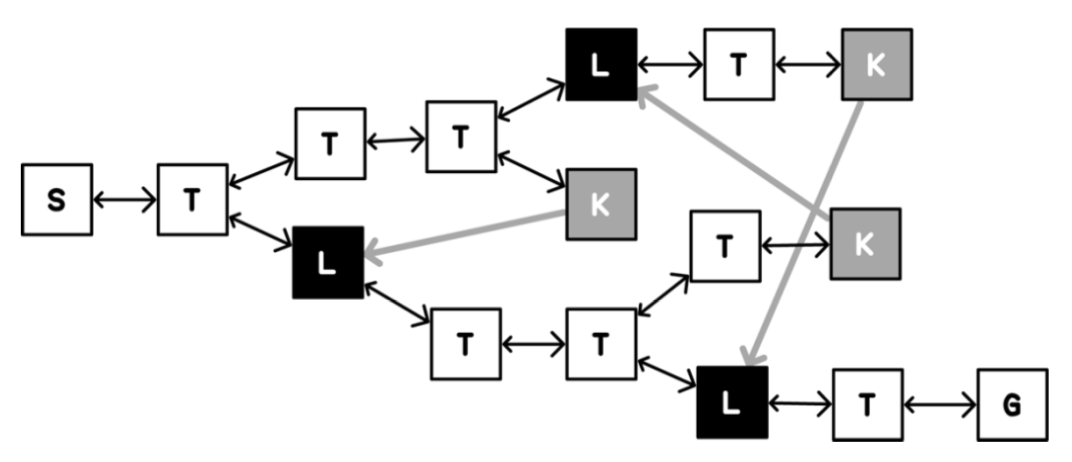
\includegraphics[width=\linewidth]{assets/mission-graph.png}
    \caption{Non-linear mission graph with tasks (T), locks (L), and keys (K) \protect\cite{Dormans2011}}
    \label{fig:mission-graph}
\end{figure}

In a straightforward way, locks represent obstacles requiring a specific key which is only available in a different part of the mission.
This also highlights the controllable strength of grammars. 
Given that the graph grammar is defined correctly it is automatically ensured that missions are solvable by organizing its elements in a valid order.
Furthermore, it is relatively simple to specify the number of times a certain task occurs and how often rules are applied.

With a structured mission in place, multiple approaches can be used to generate spaces.
Similarly to generative and graph grammars, special shape grammars are able to create spaces by following rewrite rules for shapes.
The inability of shape grammars to let multiple paths converge on the same target is remedied using an organic spring-based layout \cite{Dormans2011}.
Before the shape grammar is applied the mission graph runs through a simulation where the edges between vertices act as springs (see figure \ref{fig:organic-mission-layout}).
Overlapping edges are removed from the resulting organic layout.

\begin{figure}[H]
    \centering
    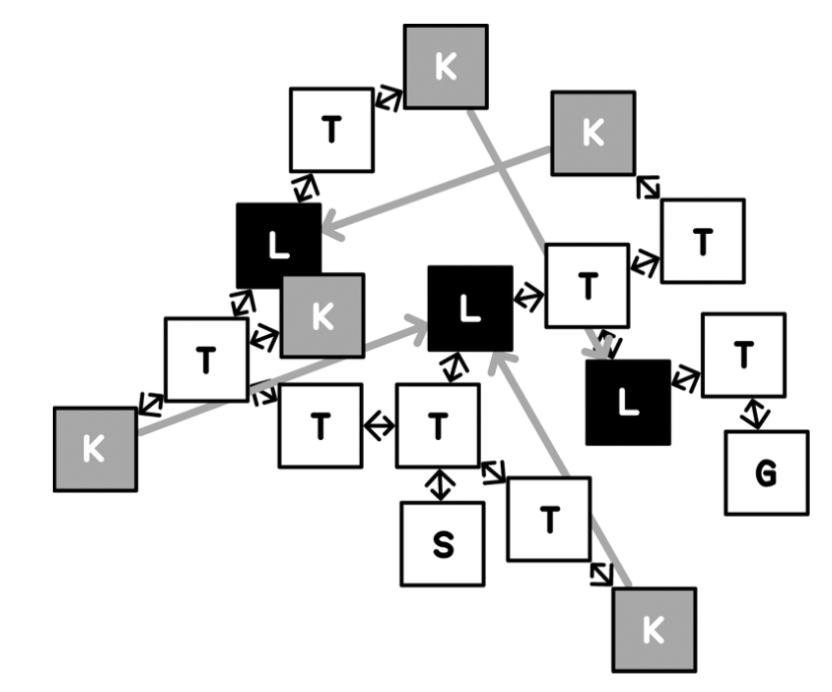
\includegraphics[width=5cm]{assets/organic-mission-layout.png}
    \caption{Organic mission graph layout \protect\cite{Dormans2011}}
    \label{fig:organic-mission-layout}
\end{figure}

Finally, player models are the crucial required component for creating adaptive games.
In their essence, they represent a player's behavior in a game.
Three distinctive approaches are identified for player modeling \cite{Dormans2011}:
\begin{itemize}
    \item \textbf{Action modeling} is used to predict actions players might take in specific situations.
    \item \textbf{Preference modeling} aims at identifying the preferences of a player leading to certain actions.
    \item \textbf{Player profiling} goes beyond modeling in the sense that it automatically creates psychologically verified player profiles. It works towards extracting traits of a player's personality.
\end{itemize}
Subsequently, player models can be exploited for adapting spaces, missions, and difficulty in games.
Features from the player model provide information for transforming the surrounding environment or changing gameplay through mission growth.
Naturally, having knowledge about the player model allows for dynamic adaption of a game's difficulty.
Usually, it is desirable to achieve a balance between the player's skills and challenge in the game.
Nevertheless, it could be used to create intentional frustratingly difficult games as well.

Being able to dynamically adapt various areas of a game is not only useful for entertainment purposes \cite{Lopes2011}.
Serious training games benefit from detailed player profiles as well.
It enables more unique and personalized experiences.
Classifying the affective state of players is not necessarily restricted to in-game actions alone.
Progression in the field of affective computing and recognition of facial, motion, and physiological features provides valuable input for adaptivity.
This allows identifying more affective states such as fun, frustration, predictability, anxiety, and boredom.
Concerning different areas of focus in research and industry efforts adapting missions and spaces is still an issue to be progressed in the future.

Detecting and recognizing facial expressions is a rather advanced field in computer vision \cite{Blom2014}. 
While this is the case actual usage for user experience analysis in non-game applications is being done in a limited number of applications.
As mentioned before relying on facial expressions for the adaption of game content is a viable solution.
It can be implemented in an unobtrusive way and in an online scenario, meaning that adaption happens while the user is playing the game.
The objective of the following scenario is to match the game's challenge with the current affective state of the player.

Facial expressions are continuously identified outputting probability distributions for seven distinct emotions: (1) neutrality, (2) happiness, (3) disgust, (4) anger, (5) fear, (6) sadness, and (7) surprise \cite{Blom2014}.
When recognition of facial expression is applied to online level generation there are two events when the affective state is used for adaption: when a player nears the end of a segment or in the case of death resetting the player to the beginning.

The Gradient Ascent Optimisation (GAO) technique is used to select appropriate level challenges.
Its objective is to minimize negative emotional responses while maximizing positive reactions.

Only neutrality, happiness, and anger are taken into account by the proposed system.
Furthermore, the authors point out that other non-verbal and verbal cues have to be recognized as well \cite{Blom2014}.
In their experimental tests, participants expressed anger using gestures and verbal actions.
\subsection{Virtual Reality} \label{sec:virtual-reality}
Virtual reality (VR) has garnered a lot of attention and hype in recent years.
It is regarded as a novelty which naturally spikes interest in people.
However, technical limitations still prevent mainstream adoption.
This leaves consumers disappointed and somewhat disillusioned about the hype in VR.
Interestingly enough the concept of VR has been established for quite some time ago with Ivan Sutherland's vision in 1965 \cite{Brooks1999}.
Working implementations have been published in 1994 with the first production systems in 1999 already.

Four technologies are crucial components for VR systems and essentially encompass the definition \cite{Brooks1999}:
\begin{itemize}
    \item Visual, aural, and haptics displays immersing the user in a virtual world. Contradicting sensory signals from the real world are blocked out.
    \item The graphics rendering systems constantly streaming images with at least thirty frames per second to simulate a fluid reality.
    \item The tracking system providing information about the position and orientation of the user's head and extremities.
    \item The system responsible for building and maintaining high fidelity of the virtual world to create a realistic experience.
\end{itemize}
While these components provide the basics for VR additional technologies are able to improve the immersive feeling including synthetic directional sound and sound fields, tactile and kinesthetic feedback (see also section \ref{sec:haptics}), specialized tracking gloves enabling better interactions with the virtual world, and finding adequate replacement interactions for their counterparts in the real world.

Multiple areas proved to be challenging for the usage of VR in production environments: rendering engines, tracking, ergonomics, and latency \cite{Brooks1999}.
The most problematic issues are solved to an acceptable degree which allowed the first consumers to get in touch with VR systems.
However, specific issues in rendering engines continue to exist and especially the ergonomics of equipment requires further improvement.
Exponentially growing power of graphics processing units (GPU) in recent years solved the most pressing matter of rendering engines.
Head-strapped displays lacking retina resolution carry the inherent problem that users are able to see the underlying grid due to the eyes being in close proximity to the display surface.
This issue will certainly be rendered obsolete with the fast-paced progression of display technology.
Ergonomics are still problematic since powerful VR systems require a wire from the worn equipment to the computational unit.
Wireless systems certainly exist but lack far behind the capability of dedicated desktop stations.
\subsection{Haptics} \label{sec:haptics}
While the world continues to being transformed by digitalization a lacking area is haptics of virtual objects.
Tactile technology has progressed with large companies such as Apple embedding the \emph{taptic engine} in all of its recent devices in order to provide tactile feedback under the marketing name \emph{force touch}.
However, the majority of feedback devices require an interactive surface or wearable haptic equipment.

AIREAL is a novelty tactile feedback system utilizing precise air vortices to create expressive sensations \cite{Sodhi2013}.
In combination with interactive displays or virtual reality (see also section x.x) it bears the potential of allowing users to feel 3D virtual objects without touching or wearing additional haptic equipment.
This fosters blurring the line between the virtual and real world.

Air vortices are created through pressure differences in a relatively small cube with a nozzle that can be freely actuated.
Their advantages are a relatively long travel distance (up to one meter), efficiency, low costs, and scalability.

Five principles steered the design of applications for the AERIAL haptics system \cite{Sodhi2013}:
\begin{itemize}
    \item \textbf{Collocation:} Visual images and tactile sensations should be collocated in space and time in the sense of an overlap between projected images and haptic feedback on the user's body.
    \item \textbf{Persistence:} Static areas and objects are able to emit fixed tactile simulations representing real physical objects.
    \item \textbf{Variance:} The haptic sensations can represent varying, rich textures in 3D space.
    \item \textbf{Continuity:} The tactile feedback can be moved continuously around the user.
    \item \textbf{Transience:} Air haptics are able to actuate real physical objects in the environment near the user.
\end{itemize}

The authors identify two main limitations of the system \cite{Sodhi2013}.
Firstly, an audible knock is produced due to the use of a high amplitude and low-frequency signal.
Secondly, while it achieves its goal of avoiding active instrumentation for the user it still requires passive instrumentation for operations in the user's environment.